\titre{Définition :} Il peut y avoir zéro ou plusieurs transitions différentes avec la même lettre à partir d'un seul état. On autorise aussi des flèches $\varepsilon$ pour changer d'état sans consommer de lettre. Le nombre d'états initiaux est illimité. \\
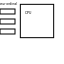
\includegraphics[width=150px]{Images/fig2.pdf} \\

\titre{Définition officielle :} Un automate non déterministe sur l'alphabet $\Sigma$ est donné par : \begin{itemize}
	\item Un ensemble fini d'états : S
	\item Une fonction de transition $f \ffonc{S\times \Sigma \cup \{\varepsilon\}}{\mathcal{P}(S)}$
\end{itemize}

\titre{Exemple : }

$$\begin{array}{r|ccc}
	\delta & \varepsilon & a & b \\ \hline
  \rightarrow 1 & \vide & \{2,3\} & \vide \\
	2 & \{3,4\} & \{2\} & \{2\} \\
  \rightarrow (3) & \vide & \{4\} & \{4\} \\
	(4) & \{3\} & \{1,2,3\} & \{4\} \\
\end{array}$$

\titre{Définition :} Un mot $w$ est accepté par un automate non déterministe s'il existe au moins un chemin qui part d'un état initial et qui arrive à un état final en suivant des transitions correspondant aux lettres de $w$, ou bien des transitions $\varepsilon$\\

\titre{Union :} Pour faire l'union de deux automates non déterministes il suffit de les mettre côte à côte.\\

\titre{Produit :} Si $A_1$ et $A_2$ sont deux automates, on cherche un automate pour les mots qui commencent par un mot de $A_1$ et continuent par un mot de $A_2$. On conserve les états initiaux de $A_1$ et les états finaux de $A_2$. On ajoute des transitions $\varepsilon$ entre les anciens états finaux de $A_1$ aux anciens états initiaux de $A_2$.\\

\titre{Etoile :} On ajoute un état qui sera le seul état initial et final, on le relie par une transition $\varepsilon$ vers tous les états initiaux et depuis tous les états finaux. \\
